\section{参数计算}
\subsection{弹簧管有关参数的确定}
\subsubsection{弹簧管外型参数的确定}
单位:(mm)
\begin{center}
\begin{tabular}{|>{\centering\arraybackslash}p{0.3\linewidth}|>{\centering\arraybackslash}p{0.3\linewidth}|>{\centering\arraybackslash}p{0.3\linewidth}|}
\hline
项目 & 公式依据 & 计算结果 \\
\hline
$x(2b=x,2a=4x)$ & $\pi(\phi-h)=\pi x+2(4x-x)$ & 5.050 \\
\hline
短轴中径$2b$ & $2b=x$ & 5.050 \\
\hline
长轴中径$2a$ & $2a=4x$ & 20.200 \\
\hline
短轴$2B$ & $2B=2b+h$ & 5.350 \\
\hline
长轴$2A$ & $2A=2a+h$ & 20.500 \\
\hline
\end{tabular}
\end{center}
\subsubsection{弹簧管末端位移的确定}
\begin{center}
\begin{tabular}{|>{\centering\arraybackslash}p{0.17\linewidth}|>{\centering\arraybackslash}p{0.03\linewidth}>{\centering\arraybackslash}p{0.5\linewidth}|>{\centering\arraybackslash}p{0.17\linewidth}|} \hline 

项目 &  \multicolumn{2}{|c|}{公式依据}& 计算结果 \\ \hline 

$\frac{\gamma-\gamma'}{\gamma}$ &  (1)&$\frac{\gamma-\gamma'}{\gamma}=p\frac{1-{\mu}^2}{E}\frac{R^2C_1}{bh[C_2+(\frac{Rh}{a^2})^2]}(1-\frac{b^2}{a^2})$& $3.07\times10^{-2}$ \\ \hline 

径向位移$S_r$ &  (2)&$S_r=\frac{\gamma-\gamma'}{\gamma}R(1-cos\gamma)$& 2.060mm \\ \hline 

切向位移$S_t$ &  (3)&$S_t=\frac{\gamma-\gamma'}{\gamma}R(\gamma-sin\gamma)$& 8.140mm \\ \hline 

总位移$S$ &  (4)&$S=\sqrt{S_r^2+S_t^2}$& 8.397mm \\ \hline 

位移方向角$\phi$ &  (5)&$\phi=arctan\frac{S_r}{S_t}$& $14.202^{\circ}$ \\ \hline

\end{tabular}
\end{center}
附:查表$C_1=0.437,C_2=0.121,\gamma=250^\circ$
\subsection{曲柄滑块机构参数的确定}
\begin{figure}[!htbp]
    \centering
    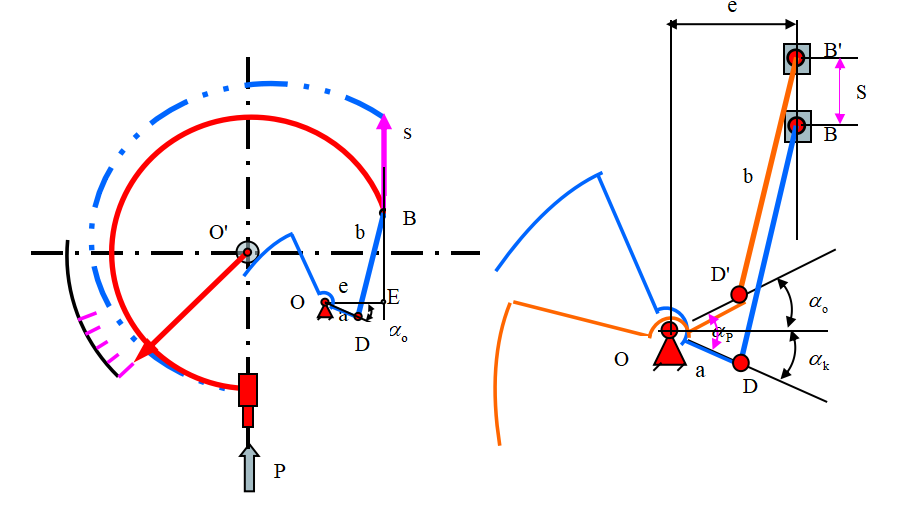
\includegraphics[width =\textwidth]{figures/4.2.1.png}
    \caption{曲柄滑块结构简图}
    \label{FIGURE4.2.1}
\end{figure}
\begin{figure}[!htbp]
    \centering
    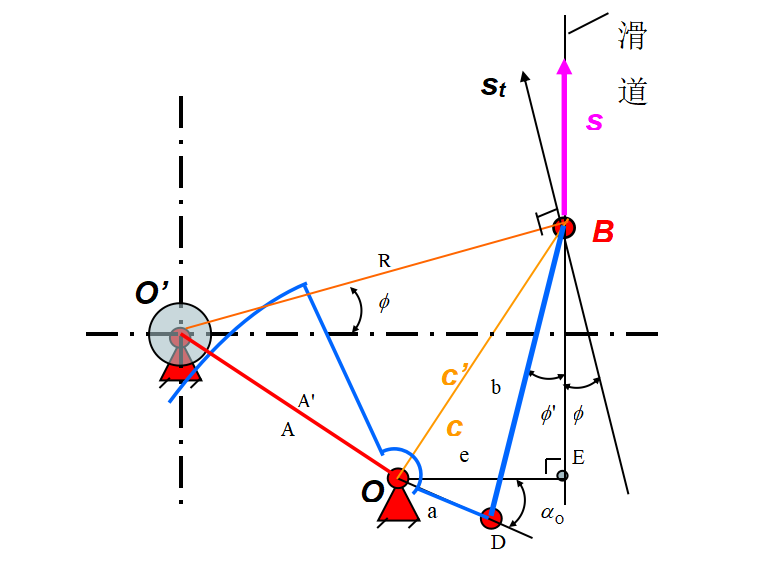
\includegraphics[width =\textwidth]{figures/4.2.2.png}
    \caption{中心距计算图}
    \label{FIGURE4.2.2}
\end{figure}
\begin{center}
\begin{tabular}{|>{\centering\arraybackslash}p{0.1\linewidth}|>{\centering\arraybackslash}p{0.7\linewidth}|>{\centering\arraybackslash}p{0.1\linewidth}|}
\hline
项目 & 公式依据 & 计算结果 \\
\hline
曲柄长度 $a$& \(\displaystyle a = \frac{s}{(\sin\alpha_k - \sin\alpha_o)+\sqrt{\lambda^2 - (\cos\alpha_o - {\varepsilon})^2}-\sqrt{\lambda^2 - (\cos\alpha_k - {\varepsilon})^2}}\)& \(9.934\)mm\\\hline
连杆初算值 $b'$& \(b' = a\lambda\)& \(38.662\)mm\\
\hline
偏移距 $e$ & \(e = a\varepsilon\) & \(9.934\)mm \\
\hline
连杆初始位与滑块运动夹角 $\phi'$ & \(\phi' = \arcsin\frac{a\cos\alpha_k - e}{b'}\) & \(1.342^\circ\) \\
\hline
${\angle}ODB$& \({\angle}ODB = 90^\circ - \alpha_k + \phi'\) & \(66.342^\circ\) \\
\hline
$c'$ & \(c' = \sqrt{a^2 + (b')^2 - 2ab'\cos\alpha_5}\) & \(36.907\)mm \\
\hline
${\angle}O'BO$ & \({\angle}O'BO = 90^\circ - \phi - \sin^{-1}\frac{e}{c'}\) & \(60.184^\circ\) \\
\hline
理论中心距 $A'$ & \(A' = \sqrt{R^2 + (c')^2 - 2Rc'\cos\alpha_7}\) & \(45.023\)mm \\
\hline
实际中心距 $A$ & (6){\qquad}\( A = \frac{mz_2}{2}(i_{21} + 1)\)& \(44.8\)mm \\
\hline
${\angle}BO'O$ & \({\angle}BO'O = \arccos\frac{R\cos\phi - e}{A} + \phi\) & \(44.861^\circ\) \\
\hline
修正后 $c$ & \(c = \sqrt{A^2 + R^2 - 2AR\cos\alpha_9}\) & 36.490mm\\
\hline
修正后 $b$ & \(b = \sqrt{a^2 + c^2 - 2ac\cos(\alpha_o + \alpha_7 + \phi)}\) & \(39.321\)mm \\
\hline
扇形角 $V_\text{齿}$& \(V_\text{齿} = \alpha_p(1 + 25\%) + 2\)个齿的度数& \(99.202^\circ\) \\ \hline
\end{tabular}
\end{center}
\subsection{齿轮传动机构有关参数的确定}
选定标准中心距$A$,由验算得$m=0.7,\,Z_2=20$时$A'$和$A$最接近,因为$Z_1=Z_2{\cdot}i_{21}=\textit{整数}$,$Z_1$不是整数无法加工。
\begin{center}
\begin{tabular}{|>{\centering\arraybackslash}p{0.6\linewidth}|>{\centering\arraybackslash}p{0.2\linewidth}|}
\hline
\text{式子} & \text{计算结果} \\ \hline
$i_{21}=5.4$& \multirow{2}{*}{$A=44.8mm$} \\ 
$A=mZ_2(1+i_{21})/2$ & \\ \hline
$Z_1=Z_2{\cdot}i_{21}$ &$ Z_1=108$\\ \hline
\multirow{6}{150pt}{\textit{设定所用齿轮为标准齿轮,用所学知识可得到右侧结果}}& $d_{a1}=15.4mm $\\ \cline{2-2}
& $d_{a2}=77.0mm$ \\ \cline{2-2}
& $d_1=14.0mm$ \\ \cline{2-2}
& $d_2=75.6mm$ \\ \cline{2-2}
& $d_{f1}=12.25mm$ \\ \cline{2-2}
& $d_{f2}=73.85mm$ \\ \hline
\end{tabular}
\end{center}
\subsection{压力表原理误差分析}
\begin{equation}
S_n = \frac{\alpha_n - \alpha_o}{\alpha_k - \alpha_o} S
\end{equation}
\begin{equation}
(7) {\quad S_n' = a(\sin\alpha_n - \sin\alpha_o) + a\sqrt{\lambda^2 - (\cos\alpha_o - \varepsilon)^2} - a\sqrt{\lambda^2 - (\cos\alpha_n - \varepsilon)^2}}
\end{equation}
\begin{center}
    \begin{tabular}{|>{\centering\arraybackslash}p{0.1\linewidth}|>{\centering\arraybackslash}p{0.15\linewidth}|>{\centering\arraybackslash}p{0.15\linewidth}|>{\centering\arraybackslash}p{0.2\linewidth}|>{\centering\arraybackslash}p{0.2\linewidth}|}
        \hline
         $\alpha_n$ & 理想值 $S_n$ & 实际值 $S_n'$ & 原理误差绝对值$|S_n-S_{n}'|$& 原理误差相对值$|S_n-S_{n}'|/S_n$\\
         \hline
         $9^\circ$ & 3.1500& 3.1499& 0.0001 & 0.003\% \\
         \hline
         $7^\circ$ & 2.8189 & 2.8208 & 0.0019 & 0.06\% \\
         \hline
         $5^\circ$ & 2.4478 & 2.4502 & 0.0024 & 0.076\% \\
         \hline
         $3^\circ$ & 2.1167 & 2.1185 & 0.0018 & 0.1011\% \\
         \hline
         $1^\circ$ & 1.7456 & 1.7462& 0.0006 & 0.0483\% \\
         \hline
         $-1^\circ$ & 1.4144 & 1.4136 & 0.0008 & 0.0461\% \\
         \hline
         $-3^\circ$ & 1.0433 & 1.0413 & 0.0020 & 0.1828\% \\
         \hline
         $-5^\circ$ & 0.7122 & 0.6896 & 0.0026 & 0.3626\% \\
         \hline
         $-7^\circ$ & 0.3611 & 0.3590 & 0.0021 & 0.5861\% \\
         \hline
         $-9^\circ$ & 0.0000 & 0.0000 & 0.0000 & 0\% \\
         \hline
    \end{tabular}
\end{center}
$\Delta = \frac{|S_n - S_n'|}{S_{max}} \times 100\%<1.5\%$,合格。
\subsection{游丝应力校核}
% Please add the following required packages to your document preamble:
% \usepackage{multirow}
\begin{center}
\begin{tabular}{|>{\centering\arraybackslash}p{0.07\linewidth}|>{\centering\arraybackslash}p{0.06\linewidth}|>{\centering\arraybackslash}p{0.5\linewidth}|>{\centering\arraybackslash}p{0.2\linewidth}|}
\hline
\multicolumn{2}{|c|}{项目}& 公式依据 & 计算结果 \\ \hline
\multicolumn{2}{|c|}{$P_1$}& \(P_1=m_\text{轴}+m_\text{帽}+m_\text{游丝}+m_\text{指针},m=\rho vg\)&$0.067N$\\ \hline
\multicolumn{2}{|c|}{$P_2$}& $P_2=m_\text{扇形齿轮}+m_\text{齿轮中心轴}$ & $0.055N$ \\ \hline
\multirow{3}{10pt}{竖直放}&$Mf_{z1}$& \(Mf_{z1}=\frac{1}{2}f_v P_1 d, f_v =0.2,\,f=0.314\)& $1.98\times10^{-5}Nm$ \\ \cline{2-3} 
 &$Mf_{z2}$&  $Mf_{z2}=\frac{1}{2}f _vP_2 d$& $1.76\times10^{-5}Nm$ \\ \cline{2-3}
 &$Mf_z$& $Mf_z =Mf_{z1}+Mf_{z2}\frac{1}{i}\frac{1}{\eta}(\eta=0.9) $& $31.28\times10^{-5}Nm$ \\ \hline
\multirow{3}{10pt}{水平放}&$Mf_{z1}$& $Mf_{z1}=\frac{1}{3}P_1 f \frac{d_1^3-d_2^3}{d_1^2-d_2^2} ,d_1=1.1d_2, f=0.2 $& $1.32\times10^{-5}Nm$ \\ \cline{2-3}
 &$Mf_{z2}$&  $Mf_{z2}=\frac{1}{3}P_2 f \frac{d_1^3-d_2^3}{d_1^2-d_2^2}$& $1.17\times10^{-5}Nm$ \\ \cline{2-3}
 &$Mf_z$& $Mf_z =Mf_{z1}+Mf_{z2}\frac{1}{i_{\textit{齿}21}}\frac{1}{\eta_{21}}  $& $2.23\times10^{-5}Nm$ \\ \hline
\multicolumn{2}{|c|}{$\max(Mf_z)$}& $\max(Mf_z\textit{竖直}, Mf_z\textit{水平})$& $31.28\times10^{-5}Nm$ \\ \hline
\multicolumn{2}{|c|}{$M_{min}$}& $(8)\quad M_{min}=\frac{kMf_z}{1-k\xi},k=2.5,\xi=0.1$ & $104\times10^{-5}Nm$ \\ \hline 
\multicolumn{2}{|c|}{$M_{\text{max}}$}& $M_{\text{max}}=M_{\text{min}}\frac{{\phi}_{max}}{{\phi}_{min}}=4M_{\text{min}}$& $416\times10^{-5}\, \text{Nm}$ \\
\hline
\multicolumn{2}{|c|}{初定游丝长$L$}& $(9){\quad }L=\pi n\frac{D_1+D_2}{2}$& $579.6\, \text{mm}$ \\
\hline
\multicolumn{2}{|c|}{初定游丝厚$h$}& $(10){\quad }h=\sqrt[4]{\frac{12LM_{\text{min}}}{\mu E \phi_{\text{min}}}},\,E = 1.1 \times 10^5 \text{MPa} $& $0.28\, \text{mm}$\\
\hline
\multicolumn{2}{|c|}{初定游丝宽$b$}& $(11){\quad }b = \mu h$& $1.7\, \text{mm}$\\
\hline
\multicolumn{2}{|c|}{最大应力$\sigma_{\text{max}}$}& $(12){\quad }\sigma_{\text{max}}=\frac{6M_{\text{max}}}{bh^2}$& $184\, \text{MPa}$\\
\hline
\multicolumn{2}{|c|}{许用应力$[\sigma_{b}]$}& $[\sigma_{b}]=\frac{\sigma_{b}}{s},\,s = 3.2,\, \sigma_{b} = 640\, \text{MPa}$& $200\, \text{MPa}$\\
\hline
\end{tabular}
\end{center}
结论:因为${\sigma}_{max}<[{\sigma}_{b}]$,因此各参数选择计算合理。
\subsection{游丝系数确定}
\begin{center}
\begin{tabular}{|>{\centering\arraybackslash}p{0.25\linewidth}|>{\centering\arraybackslash}p{0.3\linewidth}|>{\centering\arraybackslash}p{0.25\linewidth}|}
\hline
项目 & 公式依据 & 计算结果 \\ \hline
游丝长度 L & $(13)~L = \frac{Ebh^3\phi_{\text{min}}}{12M_{\text{min}}}$ & 579.6mm\\ \hline
游丝圈数 n & $(14)~n = \frac{2L}{\pi(D_1 + D_2)}$ & 9 \\ \hline
圈间距 a & $(15)~a = \frac{D_1 - D_2}{2n}$ & 1.6mm \\ \hline
游丝个数 k & $(16)~k = \frac{a}{h}$ ($k \geq 3$) & 4个 \\ \hline
\end{tabular}
\end{center}